\documentclass[14pt]{extarticle}
\usepackage{fontspec}
\usepackage{polyglossia}
\usepackage{amsmath}
\usepackage{amssymb}
\usepackage{xcolor}
\usepackage{fancyhdr}
\usepackage{graphicx}
\usepackage{listings}
\usepackage[most]{tcolorbox}
% \usepackage{setspace}
\usepackage{pifont}
\usepackage{enumitem}
\usepackage{titlesec}
\usepackage[bottom]{footmisc}
\usepackage{titling}
\usepackage{minted}
\usepackage{etoolbox}
\usepackage{array}
\usepackage{extsizes}
\usepackage{float}
\usepackage{booktabs}
\usepackage{hyperref}
\usepackage[onehalfspacing]{setspace}
\usepackage[a4paper, top=2.7cm, bottom=2.7cm, left=2.5cm, right=2.5cm, headheight=1.5cm, headsep=0.5cm]{geometry}
\usepackage{tikz}

\usetikzlibrary{automata, positioning, arrows.meta, arrows}

\newfontfamily\emoji{Segoe UI Emoji}

\pagestyle{fancy}

\setmainlanguage[numerals=western]{arabic}
\setotherlanguage{english}
% \newfontfamily\arabicfont[Script=Arabic]{Amiri}
\newfontfamily\arabicfont[Script=Arabic]{Calibri}
\newfontfamily\arabicfonttt[Script=Arabic]{Courier New}

\lstset{
  language=[Sharp]C,
  numbers=left,
  stepnumber=1,
  numbersep=8pt,
  frame=single,
  basicstyle=\ttfamily\small,
  keywordstyle=\color{blue},
  stringstyle=\color{red},
  commentstyle=\color{green!50!black}
}

\newif\ifdetailed
\ifdefined\setdetailed
  \setdetailed
\fi

\newif\ifwithsols
\ifdefined\setwithsols
  \setwithsols
\fi

% unified tcolorboxes for articles
\tcbset{colback=white, colframe=black, fonttitle=\bfseries, boxrule=0.8pt}
\newtcolorbox{boxDef}[1][]{colback=blue!5!white,colframe=blue!75!black,
  title={{\emoji📘} تعريف\ifx\\#1\\\else ~#1\fi :}}
\newtcolorbox{boxExercise}[1][]{colback=cyan!5!white,colframe=cyan!70!black,
  title={{\emoji🧩} تمرين\ifx\\#1\\\else ~#1\fi :}}
\newtcolorbox{boxExample}[1][]{colback=yellow!5!white,colframe=orange!90!black,
  title={{\emoji📝} مثال\ifx\\#1\\\else ~#1\fi :}}
\newtcolorbox{boxNote}[1][]{colback=gray!10!white,colframe=black,
  title={{\emoji✨} ملاحظة\ifx\\#1\\\else ~#1\fi :}}
\newtcolorbox{boxAttention}[1][]{colback=magenta!10!white,colframe=magenta!80!black,
  title={{\emoji🔔} تنبيه\ifx\\#1\\\else ~#1\fi :}}
\newtcolorbox{boxWarning}[1][]{colback=red!5!white,colframe=red!75!black,
  title={{\emoji⚡} ملاحظة هامة\ifx\\#1\\\else ~#1\fi :}}
\newtcolorbox{boxSolution}[1][]{colback=green!5!white,colframe=green!60!black,
  title={{\emoji✅} حل\ifx\\#1\\\else ~#1\fi :}}
\newtcolorbox{boxSymbol}[1][]{colback=purple!5!white,colframe=purple!70!black,
  title={{\emoji🔣} رمز\ifx\\#1\\\else ~#1\fi :}}
\newtcolorbox{boxHint}[1][]{colback=teal!5!white,colframe=teal!60!black,
  title={{\emoji💡} تلميح\ifx\\#1\\\else ~#1\fi :}}


\tcbset{simplecode/.style={ colback=gray!5, colframe=black!50, boxrule=0.4pt, arc=2pt, left=4pt,right=4pt,top=4pt,bottom=4pt}}
\newenvironment{boxCode}{\begin{tcolorbox}[simplecode]}{\end{tcolorbox}}

\newcolumntype{C}[1]{>{\centering\arraybackslash}p{#1}}

% redefine spaces after titles
\makeatletter
\renewcommand{\@maketitle}{%
  \begin{center}
    {\huge \bfseries \@title \par}%
    \vskip 0.2em % space between title and author
    {\large \@author \par}%
    % \vskip 0.2em % space between author and date
    % {\normalsize \@date \par}%
  \end{center}
}
\makeatother

\fancyhf{} % clear default
\fancypagestyle{plain}{
  \fancyhf{}
  \fancyhead[L]{مدرسة التسامح الشاملة}
  % \fancyhead[L]{
\includegraphics[height=1cm]{../../../images/logoTasamoh.png}}
  \fancyhead[R]{الأستاذ محمود اغبارية}
  \fancyfoot[C]{\thepage}
}

\fancyhead[L]{مدرسة التسامح الشاملة}
\fancyhead[R]{الأستاذ محمود اغبارية}
\fancyfoot[C]{\thepage}
% \date{\today}

\setcounter{tocdepth}{3} % only section subsection and subsubsection in TOC

\newcommand{\importpdfpage}[2]{%
    \thispagestyle{empty}
    \newgeometry{left=0cm,right=0cm,top=0cm,bottom=0cm}
    \includegraphics[page=#2,width=0.95\paperwidth,height=0.95\paperheight,keepaspectratio]{#1}
    \restoregeometry
}

\newcommand{\insertFullImg}[1]{%
    \noindent
    \makebox[\textwidth][c]{
        \includegraphics[width=0.9\paperwidth,keepaspectratio]{#1}%
    }%
}%

% ----------------------


% \begin{document}

% \maketitle

% % \clearpage  % start TOC on a new page
% % \renewcommand{\contentsname}{جدول المحتويات}
% % \tableofcontents
% % \clearpage

% \part*{part 1} % the * prevents numbering
% \section*{مقدمة}
% \subsection*{مثال رياضي}
% \subsubsection*{مثال فرعي}
% \paragraph*{ paragraph 1}
% \subparagraph*{sub paragraph 1}

% \ifdetailed
% \begin{english}
% \begin{minted}{csharp}
% // C# Example
% \end{minted}
% \end{english}
% \fi

% OLD WAY
% \ifdetailed
% \begin{english}
% \begin{lstlisting}
% // C# Example
% \end{lstlisting}
% \end{english}
% \fi

% % 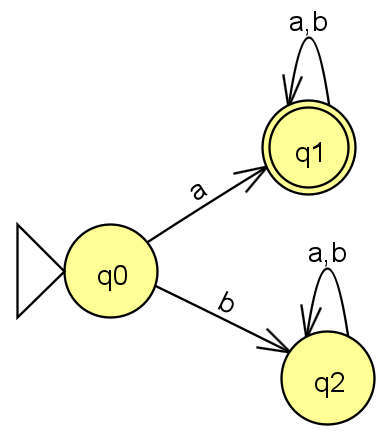
\includegraphics[width=0.2\textwidth]{../../../images/DFAs/ex1_q1.png}



% \vspace{3cm}
% \begin{flushleft}
% أرجو لكم وقتًا ممتعًا.

% الأستاذ محمود اغبارية.
% \end{flushleft}


% \end{document}


\ifwithsols
\title{حل ورقة تمرّن 11 - المصفوفة ثنائية الأبعاد}
\else
\title{ورقة تمرّن 11 - المصفوفة ثنائية الأبعاد}
\fi

\begin{document}

\maketitle
\thispagestyle{fancy}

في جميع الأسئلة التالية نعمل على المصفوفة \textenglish{mat} التالية ما لم يُذكر خلاف ذلك:

\begin{center}
\begin{english}
\begin{tabular}{c|cccc}
 & \textbf{[,0]} & \textbf{[,1]} & \textbf{[,2]} & \textbf{[,3]} \\
\hline
\textbf{[0,]} & 4  & 8  & 2  & 6  \\
\textbf{[1,]} & 1  & 5  & 9  & 3  \\
\textbf{[2,]} & 7  & 0  & 3  & 11 \\
\end{tabular}
\end{english}
\end{center}

\begin{enumerate}[itemsep=2em]

% ----------------------------------------------------------------
% سؤال 1 – قراءة القيم والأبعاد
% ----------------------------------------------------------------
\item
ما قيمة كل تعبير من التعبيرات التالية؟

\begin{enumerate}[itemsep=6pt]
    \item \textenglish{mat[1, 2]}
    \item \textenglish{mat[2, 0]}
    \item \textenglish{mat[0, 3]}
    \item \textenglish{mat.GetLength(0)}
    \item \textenglish{mat.GetLength(1)}
    \item \textenglish{mat[mat.GetLength(0)-1, mat.GetLength(1)-1]}
\end{enumerate}

\ifwithsols
\begin{boxSolution}
\begin{enumerate}[itemsep=4pt]
    \item \textenglish{mat[1, 2] = 9}
    \item \textenglish{mat[2, 0] = 7}
    \item \textenglish{mat[0, 3] = 6}
    \item \textenglish{mat.GetLength(0) = 3} \quad (عدد الصفوف)
    \item \textenglish{mat.GetLength(1) = 4} \quad (عدد الأعمدة)
    \item \textenglish{mat[2, 3] = 11} \quad (الزاوية اليمنى السفلى)
\end{enumerate}
\end{boxSolution}
\clearpage
\fi

% ----------------------------------------------------------------
% سؤال 2 – متابعة: ماذا يطبع الكود؟
% ----------------------------------------------------------------
\item
ما الناتج الذي يطبعه الكود التالي على المصفوفة \textenglish{mat}؟

\begin{boxCode}
\begin{english}
\begin{minted}{csharp}
for (int j = 0; j < mat.GetLength(1); j++)
    Console.Write(mat[0, j] + " ");
\end{minted}
\end{english}
\end{boxCode}

\ifwithsols
\begin{boxSolution}
\textenglish{4  8  2  6}

\textbf{الشرح:} الكود يُثبّت \textenglish{i = 0} ويتغير \textenglish{j} فقط — أي يطبع جميع عناصر \textbf{الصف الأول} فقط.
\end{boxSolution}
\clearpage
\fi

% ----------------------------------------------------------------
% سؤال 3 – متابعة: ماذا يطبع الكود؟
% ----------------------------------------------------------------
\item
ما الناتج الذي يطبعه الكود التالي؟

\begin{boxCode}
\begin{english}
\begin{minted}{csharp}
for (int i = 0; i < mat.GetLength(0); i++)
    Console.Write(mat[i, 2] + " ");
\end{minted}
\end{english}
\end{boxCode}

\ifwithsols
\begin{boxSolution}
\textenglish{2  9  3}

\textbf{الشرح:} الكود يُثبّت \textenglish{j = 2} ويتغير \textenglish{i} فقط — أي يطبع جميع عناصر \textbf{العمود الثالث} (\textenglish{col = 2}) من أعلى لأسفل.
\end{boxSolution}
\clearpage
\fi

% ----------------------------------------------------------------
% سؤال 4 – متابعة: ماذا يطبع الكود؟
% ----------------------------------------------------------------
\item
ما الناتج الذي يطبعه الكود التالي؟

\begin{boxCode}
\begin{english}
\begin{minted}{csharp}
int result = 0;
for (int i = 0; i < mat.GetLength(0); i++)
    for (int j = 0; j < mat.GetLength(1); j++)
        if (mat[i, j] % 2 == 0)
            result++;
Console.WriteLine(result);
\end{minted}
\end{english}
\end{boxCode}

\ifwithsols
\begin{boxSolution}
الناتج: \textenglish{5}

\textbf{الشرح:} نحسب عدد العناصر \textbf{الزوجية} في المصفوفة:
\begin{itemize}[itemsep=1pt]
    \item الصف 0: 4 ✔، 8 ✔، 2 ✔، 6 ✔ ← أربعة
    \item الصف 1: 1، 5، 9، 3 ← لا يوجد
    \item الصف 2: 7، 0 ✔، 3، 11 ← واحد
\end{itemize}
المجموع: $4 + 0 + 1 = 5$
\end{boxSolution}
\clearpage
\fi

% ----------------------------------------------------------------
% سؤال 5 – كتابة كود: أصغر قيمة
% ----------------------------------------------------------------
\item
اكتب عملية خارجية \textenglish{FindMin} تتلقى مصفوفة أعداد صحيحة ثنائية الأبعاد \textenglish{mat} وتُعيد أصغر قيمة فيها.

\begin{boxExample}
في المصفوفة \textenglish{mat} المعطاة، النتيجة: \textenglish{0}
\end{boxExample}

\ifwithsols
\begin{boxSolution}
\begin{boxCode}
\begin{english}
\begin{minted}{csharp}
public static int FindMin(int[,] mat)
{
    int min = mat[0, 0];
    for (int i = 0; i < mat.GetLength(0); i++)
        for (int j = 0; j < mat.GetLength(1); j++)
            if (mat[i, j] < min)
                min = mat[i, j];
    return min;
}
\end{minted}
\end{english}
\end{boxCode}
\textbf{الشرح:} نبدأ بافتراض أن \textenglish{mat[0,0]} هو الأصغر، ثم نمر على جميع العناصر ونحدّث \textenglish{min} كلما وجدنا قيمة أصغر.
\end{boxSolution}
\clearpage
\fi

% ----------------------------------------------------------------
% سؤال 6 – كتابة كود: معدّل عناصر المصفوفة
% ----------------------------------------------------------------
\item
اكتب عملية خارجية \textenglish{Average} تتلقى مصفوفة أعداد صحيحة ثنائية الأبعاد \textenglish{mat} وتُعيد معدّل جميع عناصرها (من النوع \textenglish{double}).

\begin{boxExample}
في المصفوفة \textenglish{mat} المعطاة: المجموع = \textenglish{59}، عدد العناصر = \textenglish{12}. \\
النتيجة: \textenglish{59.0 / 12 ≈ 4.917}
\end{boxExample}

\ifwithsols
\begin{boxSolution}
\begin{boxCode}
\begin{english}
\begin{minted}{csharp}
public static double Average(int[,] mat)
{
    int total = 0;
    int count = mat.GetLength(0) * mat.GetLength(1);
    for (int i = 0; i < mat.GetLength(0); i++)
        for (int j = 0; j < mat.GetLength(1); j++)
            total += mat[i, j];
    return (double)total / count;
}
\end{minted}
\end{english}
\end{boxCode}
\textbf{الشرح:} عدد العناصر الكلي = صفوف × أعمدة. نستخدم \textenglish{(double)} لضمان قسمة حقيقية وليس قسمة صحيحة.
\end{boxSolution}
\clearpage
\fi

% ----------------------------------------------------------------
% سؤال 7 – كتابة كود: مجموع الأعمدة
% ----------------------------------------------------------------
\item
اكتب عملية خارجية \textenglish{ColSums} تتلقى مصفوفة أعداد صحيحة ثنائية الأبعاد \textenglish{mat}، وتُعيد مصفوفة أحادية بحيث يحتوي العنصر \textenglish{j} على مجموع عناصر العمود \textenglish{j}.

\begin{boxExample}
في المصفوفة \textenglish{mat} المعطاة:
\begin{itemize}[itemsep=1pt]
    \item \textenglish{sums[0] = 4+1+7 = 12}
    \item \textenglish{sums[1] = 8+5+0 = 13}
    \item \textenglish{sums[2] = 2+9+3 = 14}
    \item \textenglish{sums[3] = 6+3+11 = 20}
\end{itemize}
\end{boxExample}

\ifwithsols
\begin{boxSolution}
\begin{boxCode}
\begin{english}
\begin{minted}{csharp}
public static int[] ColSums(int[,] mat)
{
    int rows = mat.GetLength(0);
    int cols = mat.GetLength(1);
    int[] sums = new int[cols];

    for (int i = 0; i < rows; i++)
        for (int j = 0; j < cols; j++)
            sums[j] += mat[i, j];

    return sums;
}
\end{minted}
\end{english}
\end{boxCode}
\textbf{الشرح:} الفرق عن \textenglish{RowSums}: المصفوفة المُعادة حجمها عدد \textbf{الأعمدة}، ونجمع في \textenglish{sums[j]} بدلاً من \textenglish{sums[i]}.
\end{boxSolution}
\clearpage
\fi

% ----------------------------------------------------------------
% سؤال 8 – كتابة كود: عدد العناصر الأكبر من قيمة
% ----------------------------------------------------------------
\item
اكتب عملية خارجية \textenglish{CountGreaterThan} تتلقى مصفوفة أعداد صحيحة ثنائية الأبعاد \textenglish{mat} وعدداً صحيحاً \textenglish{val}، وتُعيد عدد العناصر الأكبر تماماً من \textenglish{val}.

\begin{boxExample}
\begin{itemize}[itemsep=1pt]
    \item \textenglish{CountGreaterThan(mat, 5)} تُعيد \textenglish{5} \quad (القيم: 8، 9، 7، 6، 11)
    \item \textenglish{CountGreaterThan(mat, 0)} تُعيد \textenglish{11}
\end{itemize}
\end{boxExample}

\ifwithsols
\begin{boxSolution}
\begin{boxCode}
\begin{english}
\begin{minted}{csharp}
public static int CountGreaterThan(int[,] mat, int val)
{
    int count = 0;
    for (int i = 0; i < mat.GetLength(0); i++)
        for (int j = 0; j < mat.GetLength(1); j++)
            if (mat[i, j] > val)
                count++;
    return count;
}
\end{minted}
\end{english}
\end{boxCode}
\end{boxSolution}
\clearpage
\fi

% ----------------------------------------------------------------
% سؤال 9 – كتابة كود: إنشاء مصفوفة (تُعيد مصفوفة)
% ----------------------------------------------------------------
\item
اكتب عملية خارجية \textenglish{CreateZigZag} تتلقى عدداً صحيحاً \textenglish{n} وتُنشئ وتُعيد مصفوفة ثنائية الأبعاد مربّعة حجمها $n \times n$، بحيث يساوي كل عنصر في الصفوف الزوجية (\textenglish{i = 0, 2, 4, ...}) قيمة \textenglish{1}، وكل عنصر في الصفوف الفردية (\textenglish{i = 1, 3, 5, ...}) قيمة \textenglish{0}.

\begin{boxExample}
\textenglish{CreateZigZag(4)} تُعيد:
\begin{center}
\begin{english}
\begin{tabular}{|c|c|c|c|}
\hline
1 & 1 & 1 & 1 \\
\hline
0 & 0 & 0 & 0 \\
\hline
1 & 1 & 1 & 1 \\
\hline
0 & 0 & 0 & 0 \\
\hline
\end{tabular}
\end{english}
\end{center}
\end{boxExample}

\ifwithsols
\begin{boxSolution}
\begin{boxCode}
\begin{english}
\begin{minted}{csharp}
public static int[,] CreateZigZag(int n)
{
    int[,] mat = new int[n, n];
    for (int i = 0; i < n; i++)
        for (int j = 0; j < n; j++)
            mat[i, j] = (i % 2 == 0) ? 1 : 0;
    return mat;
}
\end{minted}
\end{english}
\end{boxCode}
\textbf{الشرح:} نستخدم \textenglish{i \% 2 == 0} للتحقق هل الصف زوجي. قيمة \textenglish{j} لا تؤثر لأن جميع عناصر نفس الصف تحمل نفس القيمة.
\end{boxSolution}
\clearpage
\fi

% ----------------------------------------------------------------
% سؤال 10 – كتابة كود: رقم الصف ذو أكبر مجموع
% ----------------------------------------------------------------
\item
اكتب عملية خارجية \textenglish{MaxRowIndex} تتلقى مصفوفة أعداد صحيحة ثنائية الأبعاد \textenglish{mat}، وتُعيد \textbf{رقم الصف} الذي يملك أكبر مجموع.

\begin{boxExample}
في المصفوفة \textenglish{mat} المعطاة:
\begin{itemize}[itemsep=1pt]
    \item مجموع الصف 0: \textenglish{4+8+2+6 = 20}
    \item مجموع الصف 1: \textenglish{1+5+9+3 = 18}
    \item مجموع الصف 2: \textenglish{7+0+3+11 = 21}
\end{itemize}
النتيجة: \textenglish{2} لأنّ الصف 2 يملك أكبر مجموع.
\end{boxExample}

\ifwithsols
\begin{boxSolution}
\begin{boxCode}
\begin{english}
\begin{minted}{csharp}
public static int MaxRowIndex(int[,] mat)
{
    int maxSum = int.MinValue;
    int maxIdx = 0;
    for (int i = 0; i < mat.GetLength(0); i++)
    {
        int rowSum = 0;
        for (int j = 0; j < mat.GetLength(1); j++)
            rowSum += mat[i, j];
        if (rowSum > maxSum)
        {
            maxSum = rowSum;
            maxIdx = i;
        }
    }
    return maxIdx;
}
\end{minted}
\end{english}
\end{boxCode}
\textbf{الشرح:} في كل دورة \textenglish{i} نحسب مجموع الصف الحالي ونقارنه بأكبر مجموع رأيناه حتى الآن. نحتفظ بـ\textenglish{maxIdx} لأن السؤال يطلب \textbf{رقم الصف} لا المجموع نفسه.
\end{boxSolution}
\clearpage
\fi

% ----------------------------------------------------------------
% سؤال 11 – كتابة كود (void): نفي المصفوفة
% ----------------------------------------------------------------
\item
اكتب عملية خارجية \textenglish{Negate} تتلقى مصفوفة أعداد صحيحة ثنائية الأبعاد \textenglish{mat}، وتُعدّل المصفوفة \textbf{مباشرةً} بضرب كل عنصر فيها بـ \textenglish{(-1)}.

\begin{boxExample}
المصفوفة \textenglish{\{\{3, -1\}, \{0, 5\}\}} تصبح \textenglish{\{\{-3, 1\}, \{0, -5\}\}}.
\end{boxExample}

\ifwithsols
\begin{boxSolution}
\begin{boxCode}
\begin{english}
\begin{minted}{csharp}
public static void Negate(int[,] mat)
{
    for (int i = 0; i < mat.GetLength(0); i++)
        for (int j = 0; j < mat.GetLength(1); j++)
            mat[i, j] *= -1;
}
\end{minted}
\end{english}
\end{boxCode}
\textbf{الشرح:} العملية من نوع \textenglish{void} لأنها تُعدّل المصفوفة الأصلية مباشرةً — المصفوفات تُمرَّر بالمرجع في \textenglish{C\#} لذا لا حاجة لـ \textenglish{return}.
\end{boxSolution}
\clearpage
\fi

% ----------------------------------------------------------------
% سؤال 12 – كتابة كود: استخراج صف كمصفوفة أحادية
% ----------------------------------------------------------------
\item
اكتب عملية خارجية \textenglish{GetRow} تتلقى مصفوفة أعداد صحيحة ثنائية الأبعاد \textenglish{mat} ورقم صف \textenglish{row}، وتُعيد مصفوفة أحادية تحتوي على عناصر ذلك الصف.

\begin{boxExample}
\textenglish{GetRow(mat, 2)} تُعيد \textenglish{\{7, 0, 3, 11\}}.
\end{boxExample}

\ifwithsols
\begin{boxSolution}
\begin{boxCode}
\begin{english}
\begin{minted}{csharp}
public static int[] GetRow(int[,] mat, int row)
{
    int cols = mat.GetLength(1);
    int[] result = new int[cols];
    for (int j = 0; j < cols; j++)
        result[j] = mat[row, j];
    return result;
}
\end{minted}
\end{english}
\end{boxCode}
\textbf{الشرح:} نُثبّت \textenglish{i = row} ونتغير في \textenglish{j} فقط. المصفوفة المُعادة أحادية وحجمها يساوي عدد الأعمدة.
\end{boxSolution}
\clearpage
\fi

% ----------------------------------------------------------------
% سؤال 13 – متابعة: تحليل كود معطى
% ----------------------------------------------------------------
\item
معطى الكود التالي:

\begin{boxCode}
\begin{english}
\begin{minted}{csharp}
public static int Mystery(int[,] mat)
{
    int res = 0;
    for (int i = 0; i < mat.GetLength(0); i++)
        for (int j = 0; j < mat.GetLength(1); j++)
            if (mat[i, j] > mat[i, 0])
                res++;
    return res;
}
\end{minted}
\end{english}
\end{boxCode}

\begin{enumerate}[itemsep=8pt]
    \item ما الذي تُعيده العملية عند تطبيقها على المصفوفة \textenglish{mat} المعطاة؟
    \item صف بكلمات بسيطة ما تفعله هذه العملية بشكل عام.
\end{enumerate}

\ifwithsols
\begin{boxSolution}
\begin{enumerate}[itemsep=6pt]
    \item \textbf{تُعيد \textenglish{6}.} \\
    نقارن كل عنصر بأول عنصر في نفس صفه (\textenglish{mat[i,0]}):
    \begin{itemize}[itemsep=1pt]
        \item الصف 0 (\textenglish{mat[0,0]=4}): 8>4 ✔، 2>4 ✗، 6>4 ✔ ← عددان.
        \item الصف 1 (\textenglish{mat[1,0]=1}): 5>1 ✔، 9>1 ✔، 3>1 ✔ ← ثلاثة.
        \item الصف 2 (\textenglish{mat[2,0]=7}): 0>7 ✗، 3>7 ✗، 11>7 ✔ ← واحد.
    \end{itemize}
    المجموع: $2+3+1 = 6$.

    \item العملية تحسب \textbf{عدد العناصر في كل صف التي تتجاوز قيمة أول عنصر في نفس الصف}.
\end{enumerate}
\end{boxSolution}
\clearpage
\fi

% ----------------------------------------------------------------
% سؤال 14 – كتابة كود: هل صفّان متساويان؟
% ----------------------------------------------------------------
\item
اكتب عملية خارجية \textenglish{AreRowsEqual} تتلقى مصفوفة أعداد صحيحة ثنائية الأبعاد \textenglish{mat} ورقمَي صفّين \textenglish{r1} و\textenglish{r2}، وتُعيد \textenglish{true} إذا كان الصفّان يحتويان على نفس القيم بنفس الترتيب، و\textenglish{false} إذا كانا مختلفَين.

\begin{boxExample}
في المصفوفة \textenglish{\{\{1,2,3\},\{4,5,6\},\{1,2,3\}\}}:
\begin{itemize}[itemsep=1pt]
    \item \textenglish{AreRowsEqual(mat, 0, 2)} تُعيد \textenglish{true}
    \item \textenglish{AreRowsEqual(mat, 0, 1)} تُعيد \textenglish{false}
\end{itemize}
\end{boxExample}

\ifwithsols
\begin{boxSolution}
\begin{boxCode}
\begin{english}
\begin{minted}{csharp}
public static bool AreRowsEqual(int[,] mat, int r1, int r2)
{
    for (int j = 0; j < mat.GetLength(1); j++)
        if (mat[r1, j] != mat[r2, j])
            return false;
    return true;
}
\end{minted}
\end{english}
\end{boxCode}
\textbf{الشرح:} حالما نجد اختلافاً بين عنصرَين في نفس العمود نُعيد \textenglish{false} فوراً. إذا انتهت الحلقة بدون اختلاف نُعيد \textenglish{true}.
\end{boxSolution}
\clearpage
\fi

% ----------------------------------------------------------------
% سؤال 15 – كتابة كود: تحويل ثنائية إلى أحادية (Flatten)
% ----------------------------------------------------------------
\item
اكتب عملية خارجية \textenglish{Flatten} تتلقى مصفوفة أعداد صحيحة ثنائية الأبعاد \textenglish{mat}، وتُعيد مصفوفة \textbf{أحادية} تحتوي على جميع عناصر المصفوفة الثنائية مرتّبةً صفاً صفاً (الصف الأول أولاً، ثم الثاني، وهكذا).

\begin{boxExample}
في المصفوفة \textenglish{mat} المعطاة، النتيجة: \\
\textenglish{\{4, 8, 2, 6, 1, 5, 9, 3, 7, 0, 3, 11\}}
\end{boxExample}

\begin{boxHint}
حجم المصفوفة الأحادية المُعادة = \textenglish{GetLength(0) * GetLength(1)}. \\
استخدم متغيراً إضافياً \textenglish{idx} لتتبّع موضع الكتابة في المصفوفة الأحادية.
\end{boxHint}

\ifwithsols
\begin{boxSolution}
\begin{boxCode}
\begin{english}
\begin{minted}{csharp}
public static int[] Flatten(int[,] mat)
{
    int rows = mat.GetLength(0);
    int cols = mat.GetLength(1);
    int[] result = new int[rows * cols];
    int idx = 0;

    for (int i = 0; i < rows; i++)
        for (int j = 0; j < cols; j++)
        {
            result[idx] = mat[i, j];
            idx++;
        }

    return result;
}
\end{minted}
\end{english}
\end{boxCode}
\textbf{الشرح:} نستخدم \textenglish{idx} كعدّاد منفصل يرتفع مع كل عنصر نكتبه في المصفوفة الأحادية. الحلقتان تضمنان المرور على العناصر بالترتيب الصحيح صفاً صفاً.
\end{boxSolution}
\fi

\end{enumerate}

\vspace{20pt}
\begin{center}
    أرجو لكم عملاً ممتعاً! / الأستاذ محمود اغبارية
\end{center}

\end{document}
